\clearpage

\section{Hoogeboom et al.: Discrete flows for compression}

\begin{notebox}
\textbf{Paper: } \fullcite{hoogeboomIntegerDiscreteFlows2019}

\hfill Notes taken: 18/2/2020 \index{February 2020}
\end{notebox}

\begin{notebox}
\tldr The idea is to use invertible flows to learn discrete distribution over digitized data (data in discrete integer space) to be able to efficiently compress using an entropy encoder over the latent $\bz = f_{ID}(\bx)$, where $f_{ID}$ is the Integer Discrete Flow. \\

The encoder doing the compression is of-the-shelf encoder (not the aim of the paper) based on the entropy principals (optimal encoding length is the Shannon information content $c = enc(z), l(c) = -\log_2 p(z)$. The important thing is to learn correctly the $p(z)$ (maximize the likelihood) so that the encoder uses the best length distribution. \\

The IDF they propose build on RealNVP combining coupling and factor-out layers with the coupling being simple additive $\bz = [\bz_a, \bz_b] = f_{ID}(\bx) = [\bx_a, \bx_{b} + round(\bt(\bx_a))]$ with rounding to ensure that they stay in integers (and no scaling to ensure the co-domain is the same as the domain).

Otherwise they use all the squeeze and permutation tricks of RealNVP.

\end{notebox}

\subsection{Intro}

\note{Based on \parencite{mackayInformationTheoryInference2005}:}

Lossless compression preserves information perfectly.
A naive way of encoding a discrete r.v. $X$ with possible outcomes (categories) $\{a_1, \ldots, a_K\}$. If we assign a unique binary code to each outcome, then the length of the codes would be the \textbf{raw bit content}\index{raw bit content} of $X$.
\begin{equation}
H_0(X) = \log_2 K
\end{equation}

Naturally, we wish to encode the data to shortest messages possible.
There is no way we can make all codes shorter but we can make some codes shorter and some longer so that on average (in expectation), the transmitted messages will be shorter.
This can be achieved if the most frequent codes (those occurring with higher probability) will be shorter and less frequent codes (those occurring with lower probability) will be longer.

\begin{definition}
Assume a random variable $X \sim p(a_i)$ generated from a discrete probability distribution $p(a_i), i=1, \ldots, K$ with $K$ possible outcomes (categories).
The \textbf{expected message length}\index{expected message length} $L(C, X)$ of encoding $C$ of the r.v. $X \sim p(a_i)$ is
$L(C, X) = \sum_{i=1}^K p(a_i) l(a_i)$, where $l(a_i)$ is the length of the encoding of the symbol (category) $a_i$.
\end{definition}

The expected message length is lower-bounded by the entropy of $X$ so that $L(C, X) \geq \rH(X) = - \sum_{i=1}^K p(a_i) \log_2 p(a_i)$ and it is optimised (minimised) if the encoding lengths are equal to the Shannon information content of the outcomes $l(a_i) = -\log_2 p(a_i)$.

If we use an encoder which assigns different lengths to the codes
\begin{equation}
l_q(a_i) = -\log_2 q(a_i) \quad \Longleftrightarrow \quad 2^{-l_q(a_i)} = q(a_i) \qquad i=1, \ldots, K \enspace ,
\end{equation}
where $q(a_i)$ is the implicit probability distribution of the encoding.
The expected message length of such an encoding is always greater than of the optimal encoding using the Shannon information content to define the lengths
\begin{align}
L(C_q, X) & = - \sum_{i=1}^K p(a_i) \log_2 q(a_i) 
= - \sum_{i=1}^K p(a_i) \log_2 \frac{q(a_i)p(a_i)}{p(a_i)}  \nn
& = - \sum_{i=1}^K p(a_i) \log_2 p(a_i) + \sum_{i=1}^K p(a_i) \log_2 \frac{p(a_i)}{q(a_i)} 
= \rH(X) + \KL{p}{q}
\end{align}
exceeding the optimal expected encoding length (the entropy $\rH(X)$) by the relative entropy (KL divergence) $\KL{p}{q}$.

\note{Back to Hoogeboom:}

To be able to encode random data $X$ efficiently, we need to learn the distribution $p(a_i)$. Maximizing the (log) likelihood $p(X)$ of the data $X$ is thus equivalent to minimizing the expected message length.

The naive idea of estimating the data distribution by simply counting the frequencies (as in a histogram) breaks down in high dimensions. 
Deep generative models allow for learning complicated data distributions.
Flow based models have advantage over other deep generative models
\begin{compactitem}
\item they admit exact log-likelihood estimation (unlike VAEs)
\item sampling (decoding) is relatively cheap \~ as expensive as inference (unlike in PixelCNNs)
\end{compactitem}

Standard flow models $f$ are defined for continuous variables. If these were to be used for compression, the latent code $z = f(x)$ would have to be quantized (discretized).
Instead they propose to work directly over the digital \emph{ordinal discrete data}\index{ordinal discrete data} such as images with 256 values per pixel, and digital video or audio to remain in the discrete domain by using \textbf{integer discrete flows} (IDF)\index{integer discrete flows}.

\begin{figure}[ht]
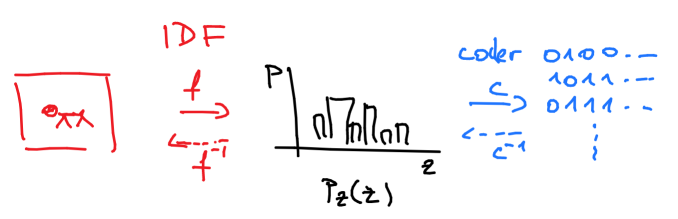
\includegraphics[width=0.7\textwidth]{idf_coding}
\centering
\caption{IDB-based lossless compression: first the data $x \sim p_x$ is passed through the learned IDF $z = f_{id}(x)$ to get to the latent $z \sim p_z$ with known distribution $p_z$, then $z$ is encoded by any off-the-shelf entropy-based encoder (e.g. Huffman, or arithmetic) into the bitstream $c$. For getting $x$ from the bistream $c$, it is first decoded (off-the-shelf) to obtain $z$ and then the inverse IDF maps it to $x = f_{id}^{-1}(z)$.}
\end{figure}

\subsection{Standard flow layers}

Normalizing flows is a stack of density transformations by the change-of-variable formula (e.g. equation \eqref{eqnice:changeOfVar}) using bijective transformations $f_i: \mX_{i} \to \mX_{i+1}$.

They consider:
\begin{compactitem}
\item \textbf{coupling layers}\index{coupling layers} as in realNVPs (section \ref{sec:realNVP}) with splitting $\bx = [\bx_a, \bx_b]$
\begin{gather}
\bz = [\bz_a, \bz_b] = f(\bx) = [\bx_a, \bt(\bx_a) + \bs(\bx_a) \odot \bx_{b}], \quad \bs(\bx_a) \neq 0 \nn
\bx = [\bx_a, \bx_b] = f^{-1}(\bz) = [\bz_{a}, (\bz_{b} - \bt(\bz_a)) \oslash \bs(\bx_a) \nn
\det \frac{\dif \bx}{\dif \bz} = \prod_{i} \bs(\bx_a)_i^{-1} \qquad p_x(\bx) = p_z(f(\bx)) \prod_{i} \bs(\bx_a)_i^{-1}
\end{gather}
\item \textbf{factor-out layers}\index{factor-out layers} also as in realNVPs (section \ref{sec:realNVP}). Here the idea is that not all the dimensions need to be propagated through all the flow layers. Instead part of the dimensions may be \emph{factored-out} at regular intervals and the rest of the flow operates over the remaining lower dimensional data.
For example for two layers we get
\begin{gather}
\bz = [\bz_1, \bz_2]: \quad [\bz_1, \by_1] = f_1(\bx) \qquad \bz_2 = f_2(\by_1) \nn
\bx = f_1^{-1}\big(\bz_1, f_2^{-1}(\bz_2)\big) \nn
p(\bz_1, \by_1) = p(\by_1) p(\bz_1 \vert \by_1) \qquad
p_y(\by_1) = p_{z_2}(f_2(\by_1)) \ \left\lvert \frac{\dif f_2(\by_1)}{\dif \by_1} \right\lvert \nn
p(\bx) = p(\bz_1, \by_1) \left\lvert \frac{\dif f_1(\bx)}{\dif \bx} \right\lvert
= p(\by_1) p(\bz_1 \vert \by_1) \left\lvert \frac{\dif f_1(\bx)}{\dif \bx} \right\lvert
= p_{z_2}(f_2(\by_1)) \ \left\lvert \frac{\dif f_2(\by_1)}{\dif \by_1} \right\lvert
p(\bz_1 \vert \by_1) \left\lvert \frac{\dif f_1(\bx)}{\dif \bx} \right\lvert \nonumber
\end{gather}
This allows for conditional dependence between parts of $\bz$
\begin{equation}
p(\bz) = p(\bz_L) p(\bz_{L-1} \vert \bz_{L})p(\bz_{L-2} \vert \bz_{L}, \bz_{L-1}) \ldots p(\bz_{1} \vert \bz_{2}, \ldots, \bz_{L})
\end{equation}

\end{compactitem}

\subsubsection{Integer discrete flows (IDF)}
For integer-valued observations $\bx \in \mX \in \mzZ^d$ and prior distribution with $p_Z(.)$ with support on $\mzZ^d$ consider a bijection $f : \mzZ^d \to \mzZ^d$ so that
\begin{equation}
p_X(\bx) = p_Z(\bz), \qquad \bz = f(\bx)
\end{equation}
IDF stacks multiple such layers. 

\paragraph{Integer discrete coupling} They design the layers to ensure that the IDF map is closed on $\mzZ^d$ so that they don't have to keep track of the co-domain of $f_{ID}$.
For $\bx = [\bx_a, \bx_b] \in \mzZ^d$
\begin{gather}\label{eqdfc:coupling}
\bz = [\bz_a, \bz_b] = f_{ID}(\bx) = [\bx_a, \bx_{b} + round(\bt(\bx_a))]\nn
\bx = [\bx_a, \bx_b] = f_{ID}^{-1}(\bz) = [\bz_{a}, \bz_{b} - round(\bt(\bx_a))]
\end{gather}
They split $a:b$ as $75\%:25\%$ to apply the rounding to fewer dimensions and have less gradient bias.
The trainable parameters are within the $\bt$ function (a network). To back-propagate through the rounding they use straight through estimator with $\nabla_x(x) = I$.

As the prior distribution $p_Z(.)$ they use the discretized logistic $DLogistic(z | \mu, \sigma)$ which assigns to an integer $z \in \mzZ$ the probability over the interval $[z - 0.5, z + 0.5]$ under the logistic distribution.
\begin{equation*}
DLogistic(z | \mu, \sigma) = \int_{z-0.5}^{z+0.5} Logistic(z' | \mu, \sigma) = F_{logistic}(z+0.5) - F_{logistic}(z-0.5) = \sigma(\frac{z+0.5-\mu}{\sigma}) - \sigma(\frac{z-0.5-\mu}{\sigma})
\end{equation*}

In the factor-out set-up we have for each factoring layer $l$ $p(z_{li} | y_{li}) = DLogistic(z_{li} | \pmb{\mu}(y_{l})_i, \pmb{\sigma}(y_{l})_i)$ where $\pmb{\mu}, \pmb{\sigma}$ are outputs of neural networks (in the implementation it is just one network spitting out $\mu$ and $\log$ scale vectors).

The latent in the last layer $z_L$ has an unconditional learned prior $DLogistic(z_{Li} | \pmb{\mu}_i, \pmb{\sigma}_i)$, where $\pmb{\mu}_i, \pmb{\sigma}_i$ are trainable parameters appearing in the loss through the likelihood evaluation. They also consider a mixture of these where they learn an additional mixing parameter $\pi_i$ (they work with 5 component mixtures.)

\subsection{Architecture}

They split the archi into levels, where each level has a \emph{squeezing operation}\index{squeezing operation}, $D integer flows$ and factor-out layer. Each integer flow consists of permutation (to ensure that all dimensions can interact with all other) followed by a discrete coupling layer. The permutations are initialised once and then kept fixed (not trained).

There is a trade-off between complexity and gradient bias influenced by the number of rounding operations. Instead of increasing the number of IDFs they make more complex the $\bt, \pmb{\mu}$ and $\pmb{\sigma}$ parts of the network.

\subsection{Experiments}

They train IDF over ImageNet32, ImageNet64 and CIFAR10 and then evaluate the likelihood and compression rate over test data ($x \to z = f_{id}(x) \to c = encode(z) \to z'=decode(c) \to x' = f_{id}^{-1}(z')$). I'm guessing the bits per dimension they mention is the $log_2$ likelihood values per pixel $d$ in the input space $\mzZ^d$ evaluated over $x'$ reconstructed from the test data $x$. The compression rate is probably the length of encodings $c$ of the test data compared to some naive encoding $c'$. Perhaps $L(c', x) = \log_2 n_{test}$?

It seems to beat the standard baselines such as JPEG, PNG, FLIF and Bit-Swap in terms of both, the log-likelihood as well as compression rate.
It even performs well if IDF is trained on other data then the the target distribution (e.g. IDF trained on ImageNet32 and used for ImageNet64 and CIFAR10) datasets.

They also have good results for compressing large images by smaller patches and in progressive decompression.

\textbf{See next page for my understanding of the implementation in their github repository.}

\subsection{My pseudo-code for implementation}
\begin{notebox}
\textbf{What I understood from the pyTorch implementation:}

For the \textbf{forward pass} you:
\begin{compactenum}
\item take $\bx$
\item $\bz \gets squeeze(\bx)$ (fixed transform)
\item repeat D times
\begin{compactitem}
\item $\bz \gets permute(\bz)$ (fixed transform)
\item $\bz \gets coupling(\bz)$ ($[\bz_a, \bz_b + \bt(\bz_a)]$ where $\bt()$ are trained neural networks, one for each D, eating on $\bz_a$ $\bz$ and spitting out an output with the same dimensions as $\bz_b$)
\end{compactitem}
\item $[\bz, \by] \gets split(\bz)$ (split $\bz$ for factoring-out parts of the dims, you won't transform $\by$ any more, $\bz$ will be further transformed)
\item $\mu, \sigma \gets h(\bz)$ where $h$ is a nn with outputs $\mu, \sigma$. These are the parameters of the conditional distribution $p(\by \vert \bz)$ (careful, here the notation is swapped as compared to the description in the paper).
\item evaluate $lpy = \log p(\by | \mu(\bz), \sigma(\bz))$ (this will enter the loss)
\item $\bx \gets \bz$ and goto 2 and repeat N-1 times
\item on the Nth repetition skip 4-6
\item evaluate $lpz = \log p(\bz | \mu, \sigma)$ where $\mu, \sigma$ are learned parameters. These are learned by maximizing the objective function $OF$
\item evaluate the loss: $OF = lpz + \sum lpy$ (the $OF$ is equal to $\log p(\bx)$ when you realize that $\bz$ and $\by$'s are different dimensions of a single latent variable living in $\mzZ^d$, the same as $\bx \in \mzZ^d$.)
\end{compactenum}

Train by standard backpropagation. Once trained, you can pass in an input $\bx$ and the $OF$ is its log-likelihood - \emph{you can evaluate the likelihood of your data points}. \\

For \textbf{sampling} you:
\begin{compactenum}
\item sample $\bz ~ p(\bz | \mu, \sigma)$, where $\mu, \sigma$ are the trained (now fixed parameters)
\item repeat D times
\begin{compactitem}
\item $\bz \gets inversecoupling(\bz)$ ($[\bz_a, \bz_b - \bt(\bz_a)]$ where $\bt()$ are the trained neural networks)
\item $\bz \gets inversepermute(\bz)$ (fixed transform)
\end{compactitem}
\item $\bz \gets unsqueeze(\bx)$ (fixed transform)
\item get parameters $\mu(\bz), \sigma(\bz) \gets h(\bz)$ where $h$ is the trained nn
\item sample $\by \sim p(\by | \mu(\bz), \sigma(\bz))$
\item stack $[\bz, \by]$ and go to 2 and repeat N times (perhaps N-1 times?)
\end{compactenum}
Once you have done this N times the length of your stackings $[\bz, \by_1, \ldots, \by_N]$ should be the same as of $\bx$ and you will get a sample of the data $\bx$ by performing the last inverse coupling, inverse permutaions and unsqueezing. \\

\textbf{Following the above pseudo-algo, I should be able to implement this. ;)}
\end{notebox}


